\begin{quote}
Participants must bring self-knowledge and no small measure of honesty
to the peer-learning project in order to accurately enunciate their
motivations.~If everyone in your peer learning project asks ``What
brings me here?'' ``How can I contribute?'' and ``How can I contribute
more effectively?'' things will really start percolating. Test this
suggestion by asking these questions yourself and taking action on the
answers!
\end{quote}

The primary motivators reported by participants in the Peeragogy project
include:

\begin{enumerate}
\itemsep1pt\parskip0pt\parsep0pt
\item
  Acquisition of training or support in a topic or field;
\item
  Building relationships with interesting people;
\item
  Finding professional opportunities through other participants;
\item
  Creating or bolstering a personal network;
\item
  More organized and rational thinking through dialog and debate {[}1{]};
\item
  Feedback about their own performance and understanding of the topic.
\end{enumerate}

We've seen that different motivations can affect the vitality of the
peeragogical process and the end result for the individual participant.~
And different participants definitely have different motivations, and
the differences can be surprising: for instance, if you're motivated by
social image, you may not be so interested in reciprocity, and vice
versa {[}2{]}. Motivations come with associated risks. For example, one
may be reluctant to mention business aspirations in a volunteer context
for fear of seeming greedy or commercial. Whether or not potential
peeragogues eventually decide to take on the risk depends on various
factors.~ Actions that typify inappropriate behavior in one culture
might represent desirable behavior in another. Motivations often come
out of the closet through conflict; for example, when one learner feels
offended or embarrassed by the actions of another.

\begin{quote}
\textbf{Philip Spalding}: ``The idea of visiting a garden together in
a group to learn the names of flowers might have been the original
intention for forming a Garden Group. The social aspect of having a
day out might be goal of the people participating.''
\end{quote}

%% 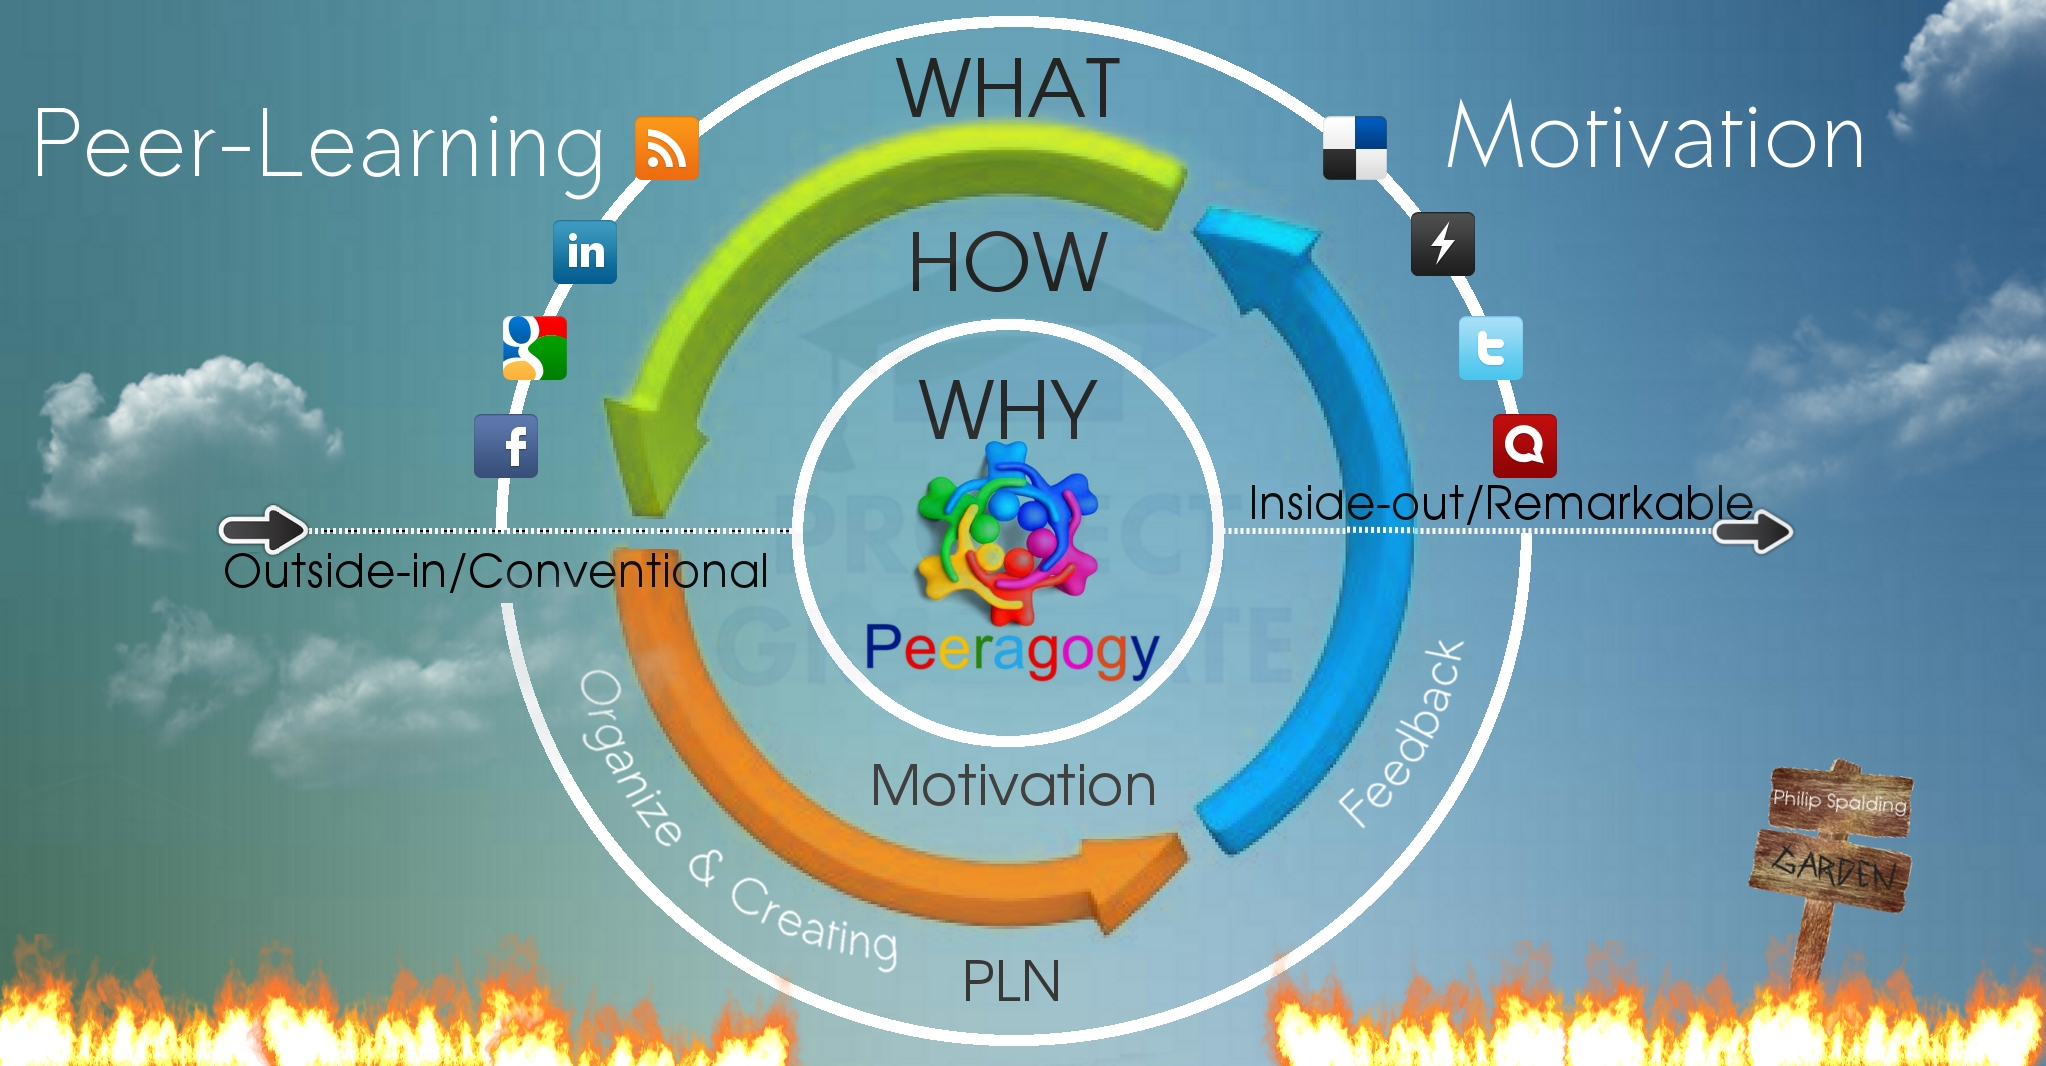
\includegraphics{http://peeragogy.org/wp-content/uploads/2013/01/44272.jpg}

%% \emph{``What's my motivation?''}

\section*{Example: Peeragogy editor Charlotte Pierce}

Basically, I'm here because as an early adopter and admitted gadget
freak, I find it fun and rewarding to explore new technologies and
topics that I feel have a practical or exciting application. But I have
some some other motivations that subtly co-exist alongside my eagerness
to explore and learn.

Howard Rheingold's reputation as an innovator and internet pioneer got
my attention when he announced his Think-Know Tools course on Facebook
in 2012. I had known of Howard from the 1990's when I was a member of
The WELL (Whole Earth `Lectronic Link). I was curious to see what Howard
was up to, so I signed onto the wiki site, paid my \$300, and took the
course starting in October.

Looking back, I realize we were practicing Peeragogy throughout the TKT
course, though at the time I hardly knew peer learning from a pickle. In
late November, missing the camaraderie and challenge of TKT, I stepped
over to check out the \emph{Peeragogy Handbook}.

Which brings me to motivations in signing on to Peeragogy. Since Howard
and several Think-Know Tools co-learners were already dedicating their
time here and their work looked innovative and exciting, I suspected
they might be onto something that I wanted to be a part of. Plus, my
brain was primed by the TKT experience. ``What if a diverse group of
people could learn a subject with little or no cost and not a lot of
barriers to entry,'' I thought. ``What if their own experience qualified
them to join, contribute, and learn.''

I also thought there might be a chance to meet some potential business
partners or clients there - but if not, the experience looked rewarding
and fun enough for me to take the risk of no direct remuneration. There
was no up front cost to me, and a wealth of knowledge to gain as a part
of something new and exciting. These are always big draws for me. I
wanted to be in on it, and nobody was telling me I couldn't!

My projections proved correct. The participants already on board were
gracious in welcoming me to Peeragogy, patient in getting me up to
speed, and persistent in coaxing me into using the tools central to the
project. I connected, learned, grew, and contributed. Now I'm on the
brink of starting a peer learning project of my own in my publishing
organization, IPNE.org. Stay tuned!

\section*{Example: Cafes, schools, workshops}

Suppose we wanted to make Peeragogy into a model that can be used in
schools, libraries, and so forth, worldwide - and, in fact we do! ~How
can we bring the basic Peeragogy motivations to bear, and make a
resource, plan of action, and process that other people can connect
with? ~In brief, how do we build peer learning into the
curriculum, providing new insight from the safety of the existing
structure?

One concrete way to implement these broad aims would be to make a
peeragogy-oriented \emph{development} project whose goal is to set up a
system of internet cafes, schools, or workshops in places like China or
Africa, where people could go to collaborate on work or to learn
technical subjects. Students could learn on the job. It seems reasonable
to think that investors could make a reasonable profit through
``franchises,'' hardware sales, and so forth -- and obviously making
money is a motivation that most people can relate to.

In developing such a project, we would want to learn from other similar
projects that already exist. ~For example, in Chicago, State Farm
Insurance has created a space called the
``\href{https://www.nextdoorchi.com/}{Next Door Cafe}'' that runs
community events. One of their offerings is free financial coaching,
with the explicit agreement that the issues you discuss return to State
Farm as market research.

\begin{quote}
\textbf{State Farm Insurance}: ``Free? Really. Yes, because we're
experimenting.  We want to learn what people really want. Then, we'll
shoot those wants back to the Farm. We help you. You help us
innovate. We're all smarter for it. We think it's a win-win.''
\end{quote}

Thus, Next Door Cafe forms part of a system to exploit the side-effects
of interpersonal interactions to create a system that learns.~ A peer
learning example from the opposite side of the world started in a slum
next to New Delhi where Sugata Mitra gave children a computer and they
self organized into a learning community and taught themselves how to
use the machine and much more.

\begin{quote}
\textbf{Sugata Mitra}: ``I think what we need to look at is we need to
look at learning as the product of educational self-organization. If
you allow the educational process to self-organize, then learning
emerges.  It's not about making learning happen. It's about letting it
happen.''
\end{quote}

In 2014, we tried a similar experiment.  We asked: Can we build a
``\href{http://commonsabundance.net/docs/help-build-the-peeragogy-accelerator-work-in-progress/}{Peeragogy
  Accelerator}'' for a half-dozen peer learning projects, each of
which defines their own metrics for success, but who come together to
offer support and guidance, using the \emph{Peeragogy Handbook} as a
resource?  We tried that with several our own projects, and benefitted
from the peer support.  Several months later, we found the Accelerator
format even more exciting when we ran a one-off series focusing on
Sagarika Bhatta's research on adaptation to climate change in Nepal.
Our sense is that peeragogy could be useful for building a global
support network around just about any project.  Peeragogy can support
a culture of real engagement, rather than ``clicktivism,'' and the
direct exchange of critically-assessed effort rather than
often-inefficient donations of cash [3].

\subsubsection{References}

\begin{enumerate}
\itemsep1pt\parskip0pt\parsep0pt
\item
  Hugo Mercier and Dan Sperber (2011). Why do humans reason? Arguments
  for an argumentative theory, \emph{Behavioral and Brain Sciences}, 34,
  57-111.
\item
  Jérôme~Hergueux (2013). \href{https://cyber.law.harvard.edu/interactive/events/luncheons/2013/11/jerome}{Cooperation
  in a Peer Production Economy: Experimental Evidence from Wikipedia},
  talk presented at the Berkman Center for Internet and Society.
\item  Kevin Edmonds (2012).
Beyond Good Intentions: The Structural Limitations of NGOs in Haiti.  \emph{Critical Sociology}, 39(3).
\end{enumerate}
